\documentclass[12pt,a4paper,english,twoside]{book}
\usepackage[english, german]{babel}
\usepackage[T1]{fontenc}
\usepackage[utf8]{inputenc}
\usepackage{amsfonts}
\usepackage{amsmath}
\usepackage{latexsym}
\usepackage{amssymb}
\usepackage{epsfig}
\usepackage{moreverb}
\usepackage{rotating}
\usepackage{enumerate}
\usepackage{graphics, graphicx,wrapfig}
\usepackage{fancybox}
\usepackage{picinpar,varioref,floatflt}
\usepackage{ae}
\usepackage{longtable}
\usepackage{textcomp}
\usepackage{float}
\usepackage{url}
\usepackage{unizhdt}
\usepackage{listings}
\usepackage{lmodern}

\graphicspath{ {content/images/} }

\setlength{\fboxsep}{3pt}%
\setlength{\fboxrule}{1pt}%

%%%%%%%%%%%%%%%%%%%%%%%%%%%%%%%%%%%%%%%%%%%%%%%%%%

% Define the language of the diploma thesis
\selectlanguage{english}
%\selectlanguage{german}

% Define available list stylings

\usepackage{color}
\definecolor{gray}{rgb}{0.4,0.4,0.4}
\definecolor{darkblue}{rgb}{0.0,0.0,0.6}
\definecolor{cyan}{rgb}{0.0,0.6,0.6}

\lstset{ % General setup for the package
	language=Perl,
	basicstyle=\small\sffamily,
	numbers=left,
 	numberstyle=\tiny,
	frame=tb,
	tabsize=4,
	columns=fixed,
	showstringspaces=false,
	showtabs=false,
	keepspaces,
	commentstyle=\color{red},
	keywordstyle=\color{blue}
}

\pagestyle{headings}

\begin{document}

%%%%%%%%%%%%%%%%%%%%%%%%%%%%%%%%%%%%%%%%%%%%%%%%%%

% Define the author printed on the cover page
\author{Reimbursement Team}

% Define the title with optional subtitle
\title{IFI Reimbursement Project}
% Define the supervisors
\supervisors{T. Bocek, A. Lareida}
% Define the submission date
\submissiondate{January 31, 2016}

% Define the students
\studentOne{Christian Davatz:}
\matOne{10-719-243}

\studentTwo{David Gallati:}
\matTwo{10-723-138}

\studentThree{Sebastian Schrepfer:}
\matThree{10-737-567}

\studentFour{Robin Engbersen:}
\matFour{08-725-202}


%%%%%%%%%%%%%%%%%%%%%%%%%%%%%%%%%%%%%%%%%%%%%%%%%%

% Make the title page
\maketitle

% Make the imprint on the back of the cover page
\makeimprint

\pagenumbering{roman}

% Include the files of the diploma thesis
\cleardoublepage
\chapter*{Abstract}
\addcontentsline{toc}{chapter}{Abstract}

\selectlanguage{german}

Kurzfassung in DE...

\selectlanguage{english}

Kurzfassung in EN...

\cleardoublepage
\chapter*{Acknowledgments}
\addcontentsline{toc}{chapter}{Acknowledgments}

Our expression of thanks goes to all the people involved in this master-project. First we like to thank Prof. Dr. Burkhard Stiller giving us the opportunity to conduct the project. Many thanks goes to Thomas Bocek and Andri Lareida for their valuable assistance. We appreciate the willingness of the reimbursement team of the communication systems department of the University of Zurich to support us with their valuable inputs.

\tableofcontents

\cleardoublepage
\pagenumbering{arabic}
\chapter{Introduction}

\section{Motivation}

The actual reimbursement process at the University of Zurich is cumbersome and contains several media disruptions. Excel documents will be created, printed, reviewed, adapted, printed and reviewed again. Numeral iterations lead to waste of paper, time and energy. Furthermore travel expenses as well as expenses need to be printed, attached, scanned and reviewed by the financial administration of each IFI department. To reduce the efforts taken for reimbursement tasks, especially on creation and review actions during the process for all participants, a new Web-based portal will be developed.

\section{Description of Work}

The aim of this project work is to design and implement a Web-based portal and its back- end functionality to operate the travel reimbursement process with a centralized and database-driven approach. The work consists of the design of a information model, the relational database model for storing reimbursement data, and the respective new travel reimbursement form. Furthermore, the development of the web portal and applications for displaying and inputting reimbursementinformation, the supervisor’s approval site, the respective financial department’s portal, and the technical administrative Web site are needed. Finally, the entire web portal and application, which shall maintain in the future the entirety of all IFI-based travel reimbursement information, shall also be tested in CSG-internal approach.


\section{Project Scope}

In our project we implement the most used features of the reimbursement process at the IFI department at the University of Zurich. This consists the complete process of creation, review, rejection, accept and print of expense elements. Besides that a synchronised interface to the existing LDAP is crucial for the user management. 
\chapter{Approach}

\section{System context}

The reimbursement-tool interacts with multiple actors and other software interfaces. In this section those interactions will be defined in detail.

\subsection{Context diagram}

The context diagram (see figure \ref{fig:context-diagram}) describes the relationships between the system and its interrogators. \textit{Creator} of expenses such as normal employees or even professors can create expenses, view and print them. However, they are not allowed to modify an expense if it's not in draft state anymore. Only \textit{Managers} and the \textit{Finance administration} is allowed to \textit{Reject expenses} back to the \textit{Creator}. Besides rejecting, they are also allowed to modify expenses after submitted by the \textit{Creator}.\newline
\textit{Guests} are allowed to view specific expenses. However, they need the 32-character long internal expense \textit{Uid} to gain access to view it. The \textit{Uid} is added on the printed expense document (see appendix \ref{sec:app-pdf} on page 2).\newline
The following sub chapters will explain why interfaces to external service providers are necessary.

\subsubsection{UZH LDAP Server}

The system fetches user-data from the UZH-IFI LDAP server (see figure \ref{fig:context-diagram}). The user-data is necessary to synchronize the user database of the reimbursement-tool with the LDAP user-data. This will allow all users, registered at the IFI LDAP server to use the system without creating a new user name and password for login. For adjusting the LDAP settings see appendix \ref{subsubsec:ldap}.

\begin{figure}[H]
    \centering
    \fbox{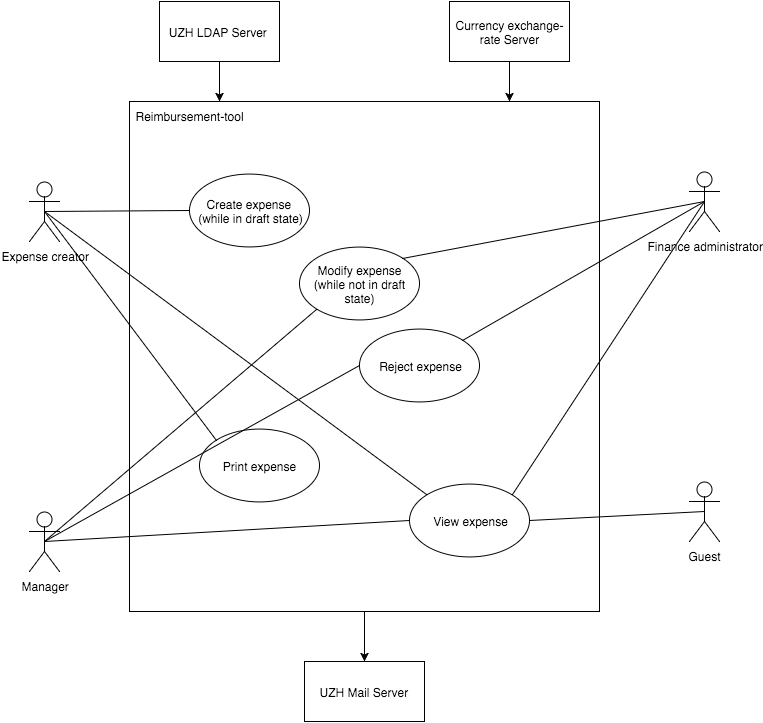
\includegraphics[width=0.80\textwidth]{context-diagram}}
    \caption{System context: Context diagram}
    \label{fig:context-diagram}
\end{figure}

\subsubsection{Currency exchange-rate Server}

To support the reimbursement-tool with accurate currency exchange-rates its necessary to access an external API providing that data. We decided to use \url{fixer.io} \cite{fixer} because it's free, it's updated daily, has a high responsibility and high availability rate. Currently the reimbursement-tool calls the API every time an exchange-rate is needed. For example if the user creates/modifies the amount of a receipt and uses a foreign currency.

\subsubsection{UZH Mail Server}
To notify participants about outstanding expense and actions that need attention, it is necessary to add an automatic mailing service. Therefor the reimbursement-tool needs to have access to the UZH Mail Server. For more information about adjusting the e-mail settings see appendix \ref{subsubsec:email}.\newpage


\section{Architecture}

The back-end is considered as the software and database running on a Tomcat \cite{tomcat} server and uses PostgreSQL \cite{postgresql} to run the database on. The system is hosted by the IFI. The front-end/client communicates with the back-end using a RESTful service interface described in section \ref{sec:restfulapi}.

\subsection{Back-end}
The back-end is developed in Java. It is structured according to the rules of a multilayered software architecture. We use the domain driven design \cite{ddd} to apply commen patterns for the layers in the backend. The domain model, that consists of the concepts, is connected to the database. Changes on the model will be automatically synchronized with the database. The service package lists all methods that are used on a domain model.\newline
DTOs (Data Transfer Object) are used to transfers data from back-end to front-end and vice verse. \newline The implemented model- and service-classes are visualized in appendix \ref{sec:app-models} and \ref{sec:app-service}. \par

\subsection{Front-end}
The front-end is developed in JavaScript using the AngularJS \cite{angular} framework. AngularJS is based on an MVC (Model View Controller) pattern. It basically consists of controllers, templates used for the view, as well as models representing the data that is shown to the user using the templates. However, AngularJS \cite{angular} extends the basic MVC concept with useful enhancements like directives, filters, injectors etc. A complete list of the available concepts in AngularJS and small examples can be found at the AgngularJS: Developer Guide \cite{angular-devguide}.

\subsection{Multilayer architecture}
We use a common \textit{Multilayer architecture} (see figure \ref{fig:architecture-layer}) in the back-end to provide a good overview and maintenance of the entire software-code. The following four layers are used:
\begin{itemize}
    \item \textbf{Presentation Layer} provides the front-end code. It uses AngularJS for the GUI creation. The \textit{Presentation Layer} interacts with the \textit{Application Layer} using RESTful services.
    \item \textbf{Application Layer} provides the available services that interact with the \textit{Business Layer}. It hosts the Security, RESTful services and the Global Exceptions.
    \item \textbf{Business Layer} provides the available services that interact with the \textit{Data Access Layer}. It provides the relevant services and models based on the \textit{Data Access Layer}.
    \item \textbf{Data Access Layer} consists of repositories and the \textit{Hybernate} database.
\end{itemize}

\begin{figure}[H]
    \centering
    \fbox{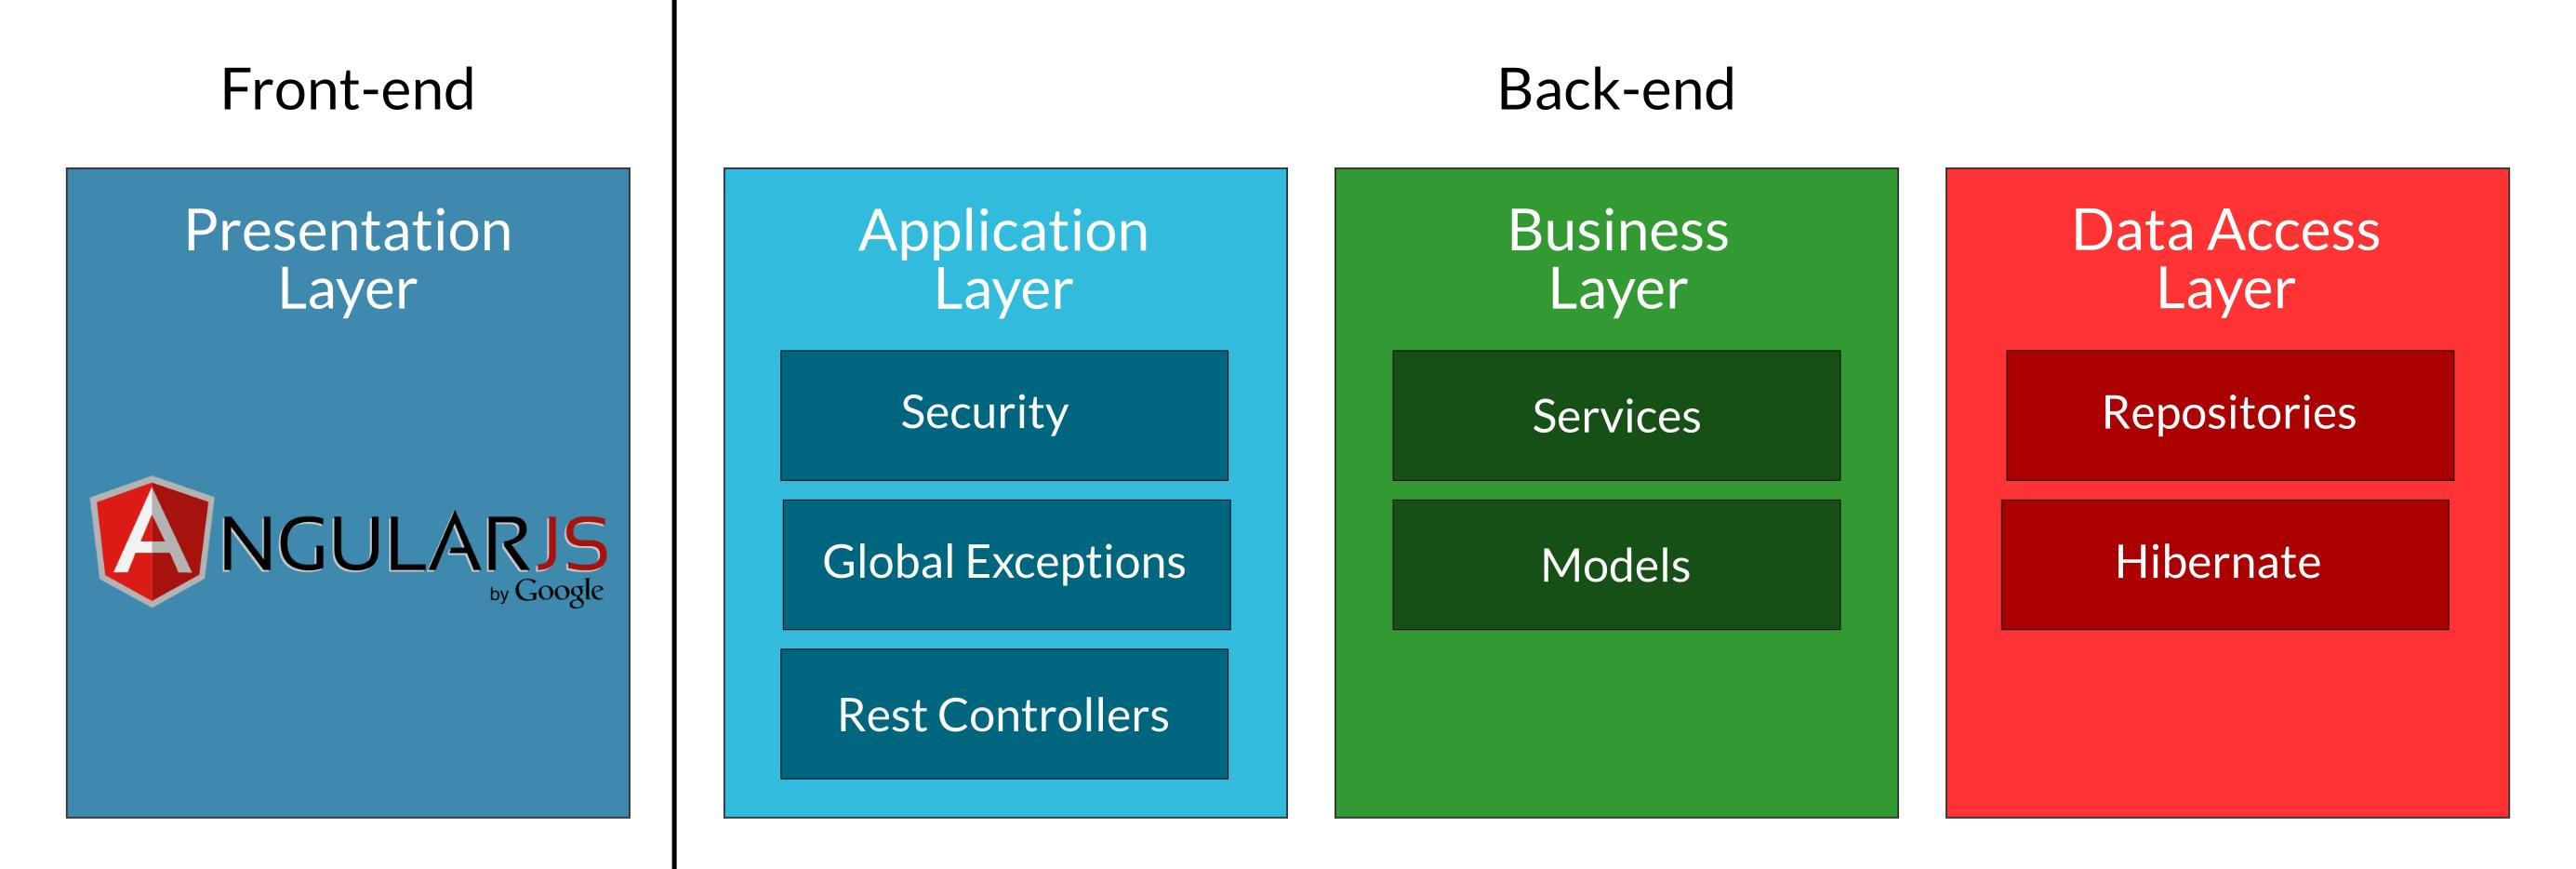
\includegraphics[width=0.80\textwidth]{architecture-layer}}
    \caption{Architecture: Multilayer architecture}
    \label{fig:architecture-layer}
\end{figure}

Our layers depend on each other while every layer communicates only with either the upper or the lower layer. This ensures a good maintainability and loose coupling of the single layers.\newline
For example: If the presentation layer needs to display an expense, the application layer will handle this request by first checking the relevant security parameter of the request followed by calling the business layer. The service will handle and aggregate the desired information fetched from the relevant models. In our case to display an expense, the service will retrieve all expense-items and expense-item-attachments.


\section{Processflow}
\label{sec:processflow}
As stated in section \ref{sec:states} an expense always has to be in one specific state. The entire process implemented in the system is documented in \ref{sec:process-diagram-rotated}.\newline
The process starts in the lane \textit{Employee}; an expense is created, receipts are added and it is forwarded to the next higher instance for verification. After the verifications by the \textit{Manager} or \textit{Department manager} and \textit{Finance administration} are successful, the signing-process will start. During the signing-process, all three entities; \textit{Employee}, \textit{Manager} and the \textit{Finance administration} need to sign the document. If all of them have signed the document correctly, the \textit{Creator} - the \textit{Employee} - can print the expense and hand it over physically to the \textit{Finance administration}. Currently this process step is not integrated in best practice. Because all of the expense receipts will be printed and after verification of the \textit{Finance administration UZH} it they will be digitalized again. This media disruption is also described in \ref{sec:future-work}.\par
However, corner-cases for example if a \textit{Manager} will act as a \textit{Creator} the expense will only be submitted to the \textit{Finance administration} for approval. However, during the signing-process the \textit{Manager} deputy has to sign as higher authority.

\subsection{States}
\label{sec:states}
During the process an expense passes through various states. An expense is always in one of the states defined followed. The State-diagram in \ref{sec:state-diagram} describes the expense transformation in viewpoint of states. Users have different roles and therefore have different authorizations to modify the state of an expense.

\begin{itemize}
    \item \textbf{DRAFT} state occurs if the expense is created and yet has not been assigned to a \textit{Manager}.

    \item \textbf{TO\_BE\_ASSIGNED} state occurs if the expense is submitted, but has not been assigned to a specific manager or the \textit{Finance administration} user. If the expense has been assigned, the expense will either have the state \newline \textbf{ASSIGNED\_TO\_MANAGER} or \newline \textbf{ASSIGNED\_TO\_FINANCE\_ADMIN}.

    \item \textbf{ASSIGNED\_TO\_MANAGER} state occurs if the expense is assigned to a specific \textit{Manager}.

    \item \textbf{ASSIGNED\_TO\_FINANCE\_ADMIN} state occurs if the expense is assigned to a specific \textit{Finance admin}.

    \item \textbf{REJECTED} state occurs if the created expense is not accepted by the \textit{Manager}, \textit{Department manager} or the \textit{Finance administration}. In \textbf{REJECTED} state the expense will be reassigned to the user who created it.

    \item \textbf{SIGNED} state occurs if the expense has been signed by all participants; \textit{Creator}, \textit{Manager} or \textit{Department manager} and \textit{Finance administration}. There exist sub states that occur if the expense is in the process of being signed:
        \begin{itemize}
            \item \textbf{TO\_BE\_SIGNED\_BY\_USER} occurs if the expense needs to be signed by the \textit{Creator}.
            \item \textbf{TO\_BE\_SIGNED\_BY\_MANAGER} occurs if the expense needs to be \newline signed by the \textit{Manager}.
            \item \textbf{TO\_BE\_SIGNED\_BY\_FINANCE\_ADMIN} occurs if the expense \newline needs to be signed by an user with role \textit{Finance administration}.
        \end{itemize}

    \item \textbf{PRINTED} state occurs if the expense and all its receipts are successfully converted into a digital document.

    \item \textbf{ARCHIVED} state occurs if the expense has been printed.
\end{itemize}

The names of the various states are coupled with the user roles. For example \textbf{ASSIGNED\_TO\_FINANCE\_ADMIN} implies that the expense is assigned to all users with roles \textit{Finance administration}.

\subsection{E-mail notification}
To inform the users of the reimbursement-tool about expense state changes, e-mail notifications have been implemented to notify affected users immediately. E-mail notifications are executed at the following actions:
\begin{itemize}
    \item An expense that has been created by a user and is assigned to a \textit{Manager}, will send an e-mail to the respective \textit{Manager}.
    \item An expense that has been approved by the \textit{Manager} and enters the state \newline \textbf{TO\_BE\_ASSIGNED}, will send an e-mail to all available users with role \textit{Finance administration}.
    \item An expense that needs to go through the signing process, will send an e-mail to notify every user who needs to sign the document.
    \item If an expense is rejected by a \textit{Manager} or the \textit{Finance administration} the \textit{Creator} of the expense will receive an e-mail notification.
\end{itemize}

E-mail notifications will be stored in a queue for each user and mailed to them three times a day in bulk mode. So we guarantee, that a user will not get spammed and the notifications messages are consolidated.

Besides state changes, e-mails will also be sent to an administrator if a general run-time exception occurs. To ensure the administrator of the reimbursement-tool is up-to date about major incidents.


\section{User roles}
\label{user-roles}

The system maps the users available in the IFI LDAP server. So every user that exists in the LDAP is capable to login to the system. He can use the same user name and password that he uses for the other University of Zurich services for login. \par

The reimbursement-tool provides different user roles. Also the roles on the reimbursement-tool are mapped with the LDAP user roles of the University of Zurich. So a user who is defined as professor for a specific group on the LDAP will be the manager for all users of this group. The reimbursement-tool provides the roles with the following authorizations to alter expenses:

\begin{itemize}
    \item \textbf{Unregistered user} are users, who are authorized to login the reimbursement-tool but have not yet completed the registration process. They have only access to the public REST services (see \ref{sec:rest-services}).
    \item \textbf{Registered user / User} passed the registration process. He can access the reimbursement-tool and create and manage his created expenses. He has one of the following roles:

    \begin{itemize}
        \item \textbf{Creator} is authorized to create and edit expenses as long as they are in DRAFT state.

        \item \textbf{Manager / Professor} are authorized to reject, accept and edit expenses as long as it is assigned to him.

        \item \textbf{Department manager} has the same authorizations as the \textit{Manager}. If a \textit{Manager} is outreach, his assignments will be forwarded to the respective \textit{Department manager}.

        \item \textbf{Finance administration} is authorized to reject, accept and edit expenses once they have been accepted by a \textit{Manager} or \textit{Department manager}. Furthermore they can manage the available cost categories and search for expenses.

        \item \textbf{Head of institute} has the same authorizations as the \textit{Manager}. In contrast to the \textbf{Department manager} there exists only one user that can be \textit{Head of institute}. The \textit{Head of institute} will have to approve the expense if, for any reason the \textit{Department manager} is not available.
    \end{itemize}
\end{itemize}


\section{Technologies}

In the following section the technologies used are being described and explained why they had been chosen.

\subsection{Back-end}

\subsubsection{Java}
The reimbursement-tool uses Java SE 7 for the back-end programming language. Java is an industry wide standard, has detailed documentation and there is sufficient knowledge at the IFI department to guarantee an adequate support and further development of the software.

\subsubsection{Hibernate}
\textit{Hibernate} abstracts the data layer. So that SQL-queries have to be written in rare cases only, which increases the code-clarity and decreases the code-complexity. All data operation are handled implicitly by defined Java data classes.\newline
H2 database is a temporary database for storing data in a database environment. It offers a simple interface and can be used for development, given that only one development database server is available. \cite{hibernate}

\subsubsection{Java Spring Framework}
We decided to use the \textit{Spring Framework} because it's well documented, widely used and easy to integrate in an existing Java project. Therefore we use various components of the Java Spring Framework \cite{spring}:
\begin{itemize}
    \item Spring Security for the login- and user-management as well as role based access-management for the RESTful resources.
    \item Spring Web MVC framework used to define RESTful interface within a few lines of code.
    \item Spring ORM used for the XML mapping within the process of Pdf-generation.
    \item Spring data is used to provide a simpler method to use data access technologies. It uses the DAO (Data Access Object) \cite{dao} to access data in a standard database like SQL.
\end{itemize}

\subsubsection{Maven}
The tool uses Apache Maven \cite{maven} for the build process and dependency management. We decided to use it, because it is widely used and is easy to maintain with a single \textit{pom.xml} file.

\subsubsection{Apache FOP}
The generated Pdf by the reimbursement-tool needs to be identical to the existing MS-Office Excel-Pdf file provided by the Finance Administration of the University of Zurich. The generated Pdf structure is added in \ref{sec:app-pdf}.\newline
The Pdf gets generated using an individual created XSLT template and a XML document generated out of a Java Object. Combining these two files generates an \textit{.fo} document, which will be used by Apache FOP \cite{apache-fop} to generate the Pdf.\par
We decided for Apache FOP because it is based on widely used standards like XML and XSL so that ongoing maintenance can be achieved easily and without specific knowledge required.

\subsubsection{Digital signature}
The ability to sign the printed Pdf document is crucial so that authenticity is provided. Especially if the Pdf document will be used as evidence by the Finance Administration of the University of Zurich. The system provides two types of signatures \cite{arx-signature}:
\begin{itemize}
    \item A \textbf{Digital signature} ensure the authenticity of the signer. Any changes made to the document after it has been signed will invalidate the signature. To use it the user has to provide his private key to successfully sign the document.
    \item \textbf{Electronic signature} does not ensure the authenticity of the signer. Anyone can theoretically make changes on the document after it has been signed without the signature become invalid. The handwritten signature captured during the registration will be stamped on the Pdf document.
\end{itemize}\par

The implementation of the digital signature is done using a third party library pdfsign.js \cite{pdfsign} that allows us to do the pdf signing in the browser and not on the server. Due to the requirement, that the private key cannot be uploaded or processed by the server, the signing needs to be done on the client using the web browser.\par

All involved participants need to sign the document; \textit{Creator}, \textit{Manager} and the \textit{Finance administration} to proof their acceptance of the expense and the captured receipts. \par

\subsection{Interface}

\subsubsection{RESTful API}
\label{sec:restfulapi}
The tool uses a RESTful API that provides services to access the back-end resources. It is implemented using the Spring MVC. /newline
The available methods provided by the backend are listed in \ref{sec:rest-services}. There exist private and public services. Private services can only be access by a \textbf{Registered user / User} (private services are marked with the term PRIVATE).

\subsubsection{Swagger UI}
The Swagger UI visualizes all methods provided by the RESTful interface using a simple GUI. Furthermore developers can interact directly with the Swagger UI to test the \texttt{HTTP} methods. Figure \ref{fig:swagger01} shows a screen-shot of our Swagger UI. It visualizes all the available methods for the \texttt{public} resource as well as the mandatory and optional parameters for \texttt{HTTP} calls. This was important for the process of development. \cite{swagger} \par
We decided on Swagger UI, because a simple and easy to understand overview, as well as a simple integration into the software source-code. Further testing the back-end functionality was very simple using Swagger UI.

\begin{figure}[H]
    \centering
    \fbox{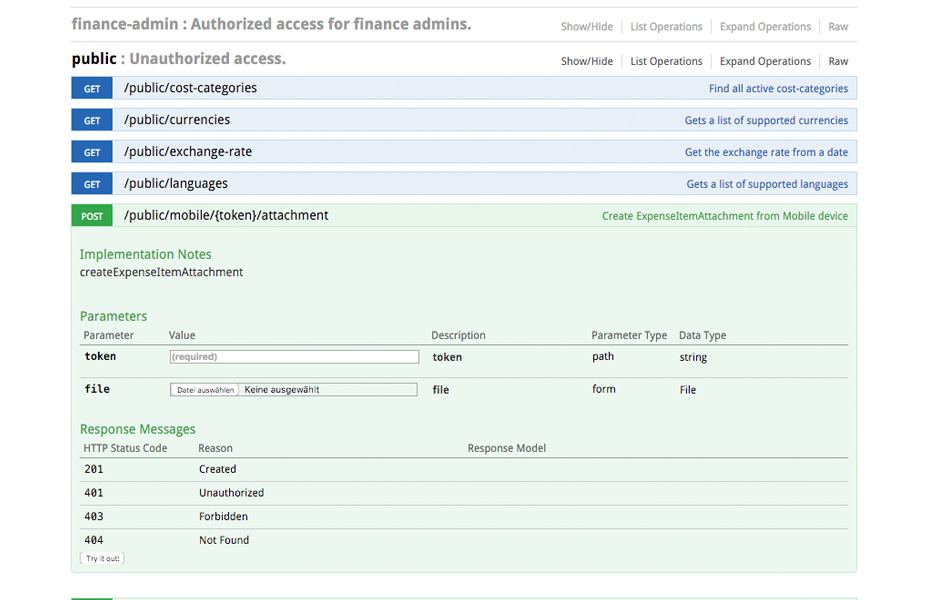
\includegraphics[width=0.80\textwidth]{swagger01}}
    \caption{Swagger: Reimbursement GUI}
    \label{fig:swagger01}
\end{figure}

\subsection{Front-end}

\subsubsection{AngularJS}
The tool uses the AngularJS framework. Its data bindings and dependency injections reduces the amount of code need to be written. Further it uses HTML templates and an sophisticated routing concept to deliver interactive GUIs. AngularJS is based on an MVC approach and is easy to integrate with REST services.\cite{angular}\par
We used AngularJS because of its broad community and the fact that it's supported by Google makes it future-proof.

\subsubsection{Bootstrap}
Bootstrap is a framework that consists of HTML, CSS and JavaScript elements. It can be used to create appealing responsive websites. Further it's CSS elements are supported by most of the desktop and mobile web-browsers available. The tool uses Bootstrap v. 3.3.5. \cite{bootstrap}\par
We use Bootstrap to speed-up the GUI development process. Using the elements it provides makes it easy to setup a responsive website within minutes. Further it provides a lot of fancy HTML/CSS elements like \textit{accordions}, \textit{modals}, etc.

\subsubsection{Bower}
The tool uses Bower for the client-side package management. Bower is a package manager for JavaScript web applications like AngularJS. It keeps track of the used assets, frameworks, libraries, etc. \cite{bower} \par
We used Bower because of its widely used, has a sound documentation and is easy to work with.

\subsubsection{Grunt}
Grunt is a JavaScript task runner. We use it for our client-side build. Its plugin directory supports a lot of modules to optimize the development work flow. Code-uglifying, concating, sass-compiling, file operations, auto prefixing etc. \cite{grunt} \par
We used Grunt because its widely used and there exists sound know how about its usage in our team.

%\input{.tex}
%\input{.tex}
\chapter{Conclusions}

\section{Summary}

The reimbursement process at the IFI department of the University of Zurich was based on a single MS-Office Excel file that has been used to capture the receipt expenses and pass them physically through the entire reimbursement process. For the participants it was difficult because they had to pass the digital Excel file and the physical receipts to the next member in the process. The extra effort needed and increasing digitization of the employees leads to the idea to digitize the entire process by a single system.\newline
It was developed in order to reduce the effort needed of the participants in the process and to increase the efficiency and flexibility in capturing receipts, by allowing the user to add them on the go using a smart phone. Besides that, the Finance Administration of the IFI department will get analytical tools to gain a better insight knowledge of the state-distribution of expense while in the reimbursement process. The integrated search engine allows them to search and retrieve archived expenses within seconds. \par
Overall the system works. Expenses can be created, modified, deleted and passed during the entire process. They can be printed as a Pdf. The Pdf document fulfill all requirements of the Finance Administration of the IFI. However, there are still some open tasks need to be done in the future to improve the embedding of the systems into the environment. 


\section{Future work}
\label{sec:future-work}

The current implementation of the reimbursement-tool covers the basic features to run the entire reimbursement-process at the IFI digitally. However, there is still some future work to be done, which will be addressed in the following subsections. 

\subsection{Digital signature}
Currently the private key for the digital signature has to be copy/pasted manually by the user to sign a document digitally. This needs to be improved in a way, that the private key will be loaded automatically and without any copy/paste actions. The current implementation of the WebCrypto Key Discovery API does not allow the discovery of private keys due to privacy issues with those keys \cite{webcrypto}. \par
We look forward, that those described changes will be implemented in the near future to improve the signing use case.

\subsection{Pdf version 1.5}
During the development of the reimbursement-tool a new version of the Pdf document, that needs to be delivered to the Finance Administration of the University of Zurich, was published. Obviously the new requirements need to be implemented in a future step. 

\subsection{Process integration to UZH}
Currently the expenses will be printed and delivered to the Finance Administration of the University of Zurich in paper format. In turn they'll be scanned to be digitalized and archived at the Finance Administration of the University of Zurich. If this media disruption could be suspended, the overall process efficiency increases.



\begin{thebibliography}{99}
\addcontentsline{toc}{chapter}{Bibliography}

\bibitem{fixer} Foreign exchange rates and currency conversion JSON API, URL \url{http://fixer.io/}, last visited Dec. 13, 2015
\bibitem{tomcat} Apache Tomcat - Welcome!, URL \url{http://tomcat.apache.org/}, last visit Dec. 13, 2015.
\bibitem{postgresql} PostgreSQL: The world's most advanced open source database, URL \url{http://www.postgresql.org/}, last visit Dec. 13, 2015.
\bibitem{ifi} UZH - Department for Informatics, URL \url{http://www.ifi.uzh.ch/}, last visit Dec. 3, 2015.
\bibitem{ddd} An Introduction to Domain Driven Design, URL \url{http://www.methodsandtools.com/archive/archive.php?id=97}, last visited Dec. 6, 2015
\bibitem{angular-devguide} AngularJS: Developer Guide, \newline URL \url{https://docs.angularjs.org/guide/concepts#model}, last visited Dec. 14, 2015
\bibitem{hibernate} Hibernate. Everything data. - Hibernate, URL \url{http://hibernate.org/}, last visit Nov. 18, 2015.
\bibitem{spring} Spring, URL \url{https://spring.io/}, last visit Nov. 18, 2015.
\bibitem{maven} Maven – Welcome to Apache Maven, URL \url{https://maven.apache.org/}, last visit Nov. 18, 2015.
\bibitem{dao} Core J2EE Patterns - Data Access Object, \newline URL \url{http://www.oracle.com/technetwork/java/} \newline \url{dataaccessobject-138824.html}, last visit Dec. 5, 2015
\bibitem{mockito} mockito.org, URL \url{http://mockito.org/}, last visit Nov. 18, 2015.
\bibitem{apache-fop} Apache(tm) FOP - a print formatter driven by XSL formatting objects (XSL-FO) and an output independent formatter., URL \url{https://xmlgraphics.apache.org/fop/}, last visit Dec. 12, 2015.
\bibitem{pdfsign} Communication-Systems-Group/pdfsign.js, \newline URL \url{https://github.com/Communication-Systems-Group/pdfsign.js}, last visit Jan. 21, 2016.
\bibitem{swagger} Swagger | The World's Most Popular Framework for APIs, URL \url{http://swagger.io/}, last visit Nov. 18, 2015.
\bibitem{angular} AngularJS Documentation for introduction, URL \url{https://docs.angularjs.org/guide/introduction}, last visit Nov. 18, 2015.
\bibitem{bootstrap} BootstrapDocs - Twitter Bootstrap Documentation Archive,\newline URL \url{http://bootstrapdocs.com/v3.3.5/docs/}, last visit Nov. 18, 2015.
\bibitem{bower} Bower, URL \url{http://bower.io/}, last visit Nov. 18, 2015.
\bibitem{grunt} Grunt: The JavaScript Task Runner, URL \url{http://gruntjs.com/}, last visit Nov. 18, 2015.
\bibitem{webcrypto} WebCrypto Key Discovery, \newline URL \url{http://www.w3.org/TR/webcrypto-key-discovery/}, last visit Dec. 12, 2015.
\bibitem{node} Node.js, URL \url{https://nodejs.org/en/}, last visit Nov. 18, 2015.
\bibitem{arx-signature} Learn about Digital Signatures and Electronic Signatures, URL \url{http://www.arx.com/learn/about-digital-signature/digital-signature-faq/}, last visit Dec. 5, 2015




\end{thebibliography}

\chapter*{Glossary}
\addcontentsline{toc}{chapter}{Glossary}
\markboth{GLOSSARY}{}


\begin{description}
    \item[API] is an abbreviation for Application Programming Interface in computer programming. It can be used to access services of external software using an interface.
    \item[Build process] Is a process to generate a software artifact that contains the complete software code.  
    \item[Client] is the physical hardware entity that a normal user uses i.e. Personal Computer.
    \item[CSS] is an abbreviation for Cascading Style Sheets. It is used to format and style plain HTML code. 
    \item[Dependency management] is used to ensure that the compatibility between various packages is supported.
    \item[Expense] is, in the context of this document an entity that consists out of 1 - 15 receipts. It is the digital counterpart to the physical expense.
    \item[Finance Administration of Zurich] is the head of all finance administration departments of the University of Zurich.
    \item[GUI] is an abbreviation for Graphical User Interface. 
    \item[HTTP] is an abbreviation for Hypertext Transfer Protocol. The protocol is used to transmit HTML data between the client and the server.
    \item[HTML] is an abbreviation for Hypertext Markup Language. It is used to structure digital documents with content like text, images and hyperlinks. 
    \item[IFI] is an abbreviation for the Department of Informatics at the University of Zurich.
    \item[Java] is a widely used object-oriented programming language.
    \item[LDAP] is an abbreviation for Lightweight Directory Access Protocol. It's a network protocol that is used to access and manage distributed directory access and user authorization information. 
    \item[Media disruption] occurs, when a digital document is printed and transferred back to a digital format by hand.
    \item[MVC] is an abbreviation for Model View Controller. It is a widely used software pattern.
    \item[Pdf] is an abbreviation for Portable Document Format. It is a widely used file format, to present documents in most operating system in a fixed layout.
    \item[Receipt] is, in the context of this document the digital counterpart of a physical receipt.
    \item[Reimbursement-tool] is the developed prototype.
    \item[RESTful] is an abbreviation for representational state transfer in computing. Its a definition, on how to access web-based resources in the right way.
    \item[SQL] is an abbreviation for Structured Query Language. It is used to execute database calls to retrieve data in relational databases.
    \item[UI] is an abbreviation for User Interface. 
    \item[UZH] is an abbreviation for University of Zurich.
    \item[XML] is an abbreviation for Extensible Markup Language. It defines a set of rules that are machine and human readable.
    \item[XSL] is an abbreviation for Extensible Stylesheet Language. It is used to transform and render XML documents.
    \item[XSLT] is an abbreviation for Extensible Stylesheet Language Transformations. It is a special language used to transform XML documents.
    \item[MLA] is an abbreviation for Multilayered Architecture. It is an architectural software design pattern enforcing the Separation of Concerns.
    \item[SOC] is an abbreviation for Separation of Concerns. It is a design principle for separating a computer program into distinct sections, such that each section addresses a separate concern\cite{soc}.
\end{description}


%\addcontentsline{toc}{chapter}{List of Figures}
%\listoffigures
%\addcontentsline{toc}{chapter}{List of Tables}
%\listoftables

\appendix

\chapter{Installation}
\label{chap:installation}

\section{Back-end / Server}
\label{sec:backend-server}

In the following chapters the installation of the back-end is described. The back-end uses Mave for its dependency management and build process. A local Tomcat server needs to be installed and the project needs to be configured as a Maven project.

\subsection{Maven installation}
To install Maven and build the system complete the following steps:

\begin{enumerate}
    \item Maven should be already integrated in Eclipse for Java EE. If the following steps do not work, download maven and the m2e eclipse plugin.
    \item Clone or checkout the public reimbursement-server repository hosted on Github (see appendix \ref{github-source}).
    \item After checking out the server project, the project needs to be configured as a Maven project.
    \item Run \texttt{mvn:install} to build and download all the dependencies required for the project. 
    \item Download Apache Tomcat 8.0. Add the servers-view in Eclipse and click the link to create a new server. Create a new Tomcat server and add the reimbursement-server package to it.
    \item Set the port of the Tomcat to 80 instead of 8080.
\end{enumerate}

\subsection{General settings}

In the general settings section overall configuration parameters are defined and explained.

\subsubsection{LDAP}
\label{subsubsec:ldap}

Currently the synchronisation interval is defined to take part every 300 Seconds. By changing the value of \textit{reimbursement.ldap.refreshRate} on the file \texttt{application.properties} stored at the back-end in the directory \textit{src/main/resources}. \par
During the development and integration a specific file will be loaded that defines the available demo user-accounts for the reimbursement-tool. Those users are defined in the file \texttt{development-server.ldif}. The following users exist:
\begin{itemize}
\item \texttt{junior} has similar rights, just like the \textit{JuniorAssistants} group defined in the IFI LDAP tree.
\item \texttt{senior} has similar rights, just like the \textit{SeniorAssistants} group defined in the IFI LDAP tree.
\item \texttt{prof} has similar rights, just like the \textit{Professors} group defined in the IFI LDAP tree.
\item \texttt{fadmin} \& \texttt{fadmin2} \& \texttt{depman} \& \texttt{headinst} has similar rights, just like the \textit{Administration} group defined in the IFI LDAP tree.
\end{itemize}

For all the demo user-accounts, the password is \textit{password}. So to login to the system while in development select one user account and use the password. 

\subsubsection{E-mail server}
\label{subsubsec:email}

The currently used e-mail settings can be adjusted at the \texttt{application.properties} file in the back-end. E-mail templates are stored in the directory \textit{src/main/resources/email}.

\subsubsection{Pdf generation}
\label{subsubsec:pdf-xml-mappings}

The \textit{.xsl} file is used to generate an \textit{.fo} file out of an xml-file that consists of object data. In the folder \textit{src/main/resources} exists a \texttt{xml-mapping.xml} file that maps a data-object to a xml-object. The xml-object is required by the \texttt{xml2fo.xsl} and \texttt{attachmentXml2fo.xsl}. Those files transfer the xml-object into a \textit{.fo} file which is needed by the Apache FOP to generate the Pdf.  


\section{Frontend / Client}

\subsection{Basic setup}
To run the application locally on the client npm needs to be installed. If it is already installed on your system, you can skip it.

First we need to install npm and Bower:
\begin{enumerate}
  \item Make sure, you have installed the latest version of Node.js.
  \item Clone or checkout the public reimbursement-client repository hosted on Github (see appendix \ref{github-source}).
  \item Open a command-line tool and navigate to the root of the reimbursement-client directory and run \texttt{npm install}. This will download all required dependencies that are defied in the \textit{package.json}.
  \item If Bower is not already installed on your system (check in with \texttt{which bower}), install it by running \texttt{npm install -g bower}. After you have verified that Bower is installed run \texttt{bower install}. This will download all required dependencies that are defied in the \textit{bower.json}.
\end{enumerate}

\subsubsection{Grunt}
Grunt builds the front-end files. It has multiple modules to build: you can concat, copy, prefix, sass-compile etc. The configuration of Grunt is stored in \textit{Gruntfile.js} and the modules of grunt are loaded using npm.
\begin{enumerate}
  \item After all the steps in npm section are completed, grunt needs to be installed. This can be done by \texttt{npm install -g grunt-cli}. Now we can start using the grunt CLI. There are various options available:
  \begin{itemize}
      \item \texttt{grunt}: This command starts the default grunt operation. It is used to build all the files. Use it only for development purpose, because the minified versions are not created.
      \item \texttt{grunt prod}: This command minifies and uglifies all the files. Use it to test if minification and uglification covers all the production requirements.
      \item \texttt{grunt serve}: This command starts a local http-server and updates automatically. If a source file is changed, the build will be executed and the browser will be reloaded to visualize the changes.
      \item \texttt{grunt prod-serve}: This command runs starts a local server with the production files as a base.
      \item \texttt{grunt deploy}: This command builds the project with the production profile and uploads the build files to the Tomcat instance (makes a redeploy). The deployment requires a deploy.json with the server configuration. See section Deployment for details.
    \end{itemize}
\end{enumerate}

\section{Deployment}

\subsection{Backend}

To deploy the software from the local running copy to the server running a Tomcat the following steps are required:

\begin{itemize}
    \item Configure the local Java environment to run the project described in section \ref{sec:backend-server} 
    \item Store the credentials of the Tomcat instance and productive database in the maven directory. The maven directory is stored mostly on the local machines user directory in the \texttt{.m2/settings.xml} file. The file needs to have the following structure:

    \begin{lstlisting}
    <settings xmlns="http://maven.apache.org/SETTINGS/1.0.0"
        xmlns:xsi="http://www.w3.org/2001/XMLSchema-instance"
        xsi:schemaLocation="http://maven.apache.org/SETTINGS/1.0.0
        http://maven.apache.org/xsd/settings-1.0.0.xsd">
    	<servers>
    		<server>
    			<id>reimbursement-server</id>
    			<username></username>
    			<password></password>
    		</server>
    	</servers>
    
    	<profiles>
    		<profile>
    			<id>reimbursement_int</id>
    			<properties>
    				<jdbc.username></jdbc.username>
    				<jdbc.password></jdbc.password>
    			</properties>
    		</profile>
    		<profile>
    			<id>reimbursement_prod</id>
    			<properties>
    				<jdbc.username></jdbc.username>
    				<jdbc.password></jdbc.password>
    			</properties>
    		</profile>
    	</profiles>
    </settings>
    \end{lstlisting}
    
    Add the respective user name and password values to login properly.
    
    \item To configure the deployment right click to the server project in Eclipse -> Run As -> Maven Build... and enter the following values in the corresponding input fields:
    \newline
    Name: \texttt{reimbursement-deploy}
    \newline
    Goals: \texttt{clean tomcat7:redeploy}
    \newline
    Profiles: \texttt{reimbursement\_prod}
    \item Call the new created maven build and the project will be deployed to the production server.  
    
\end{itemize}
    
\subsection{Frontend}

\begin{itemize}

    \item Create a new file with the following content named \textit{deploy.json}:
    \begin{lstlisting}
        {
            "username": "",
            "password": "" 
        }   
    \end{lstlisting}
    \item Add the credentials to the file deploy.json. The deploy.json file is stored in the main directory.
    \item Open a command line tool and run \texttt{grunt deploy}. This will automatically deploy the frontend to the server. 

\end{itemize}

\chapter{}

\section{Models}
\label{sec:app-models}

\begin{figure}[H]
    {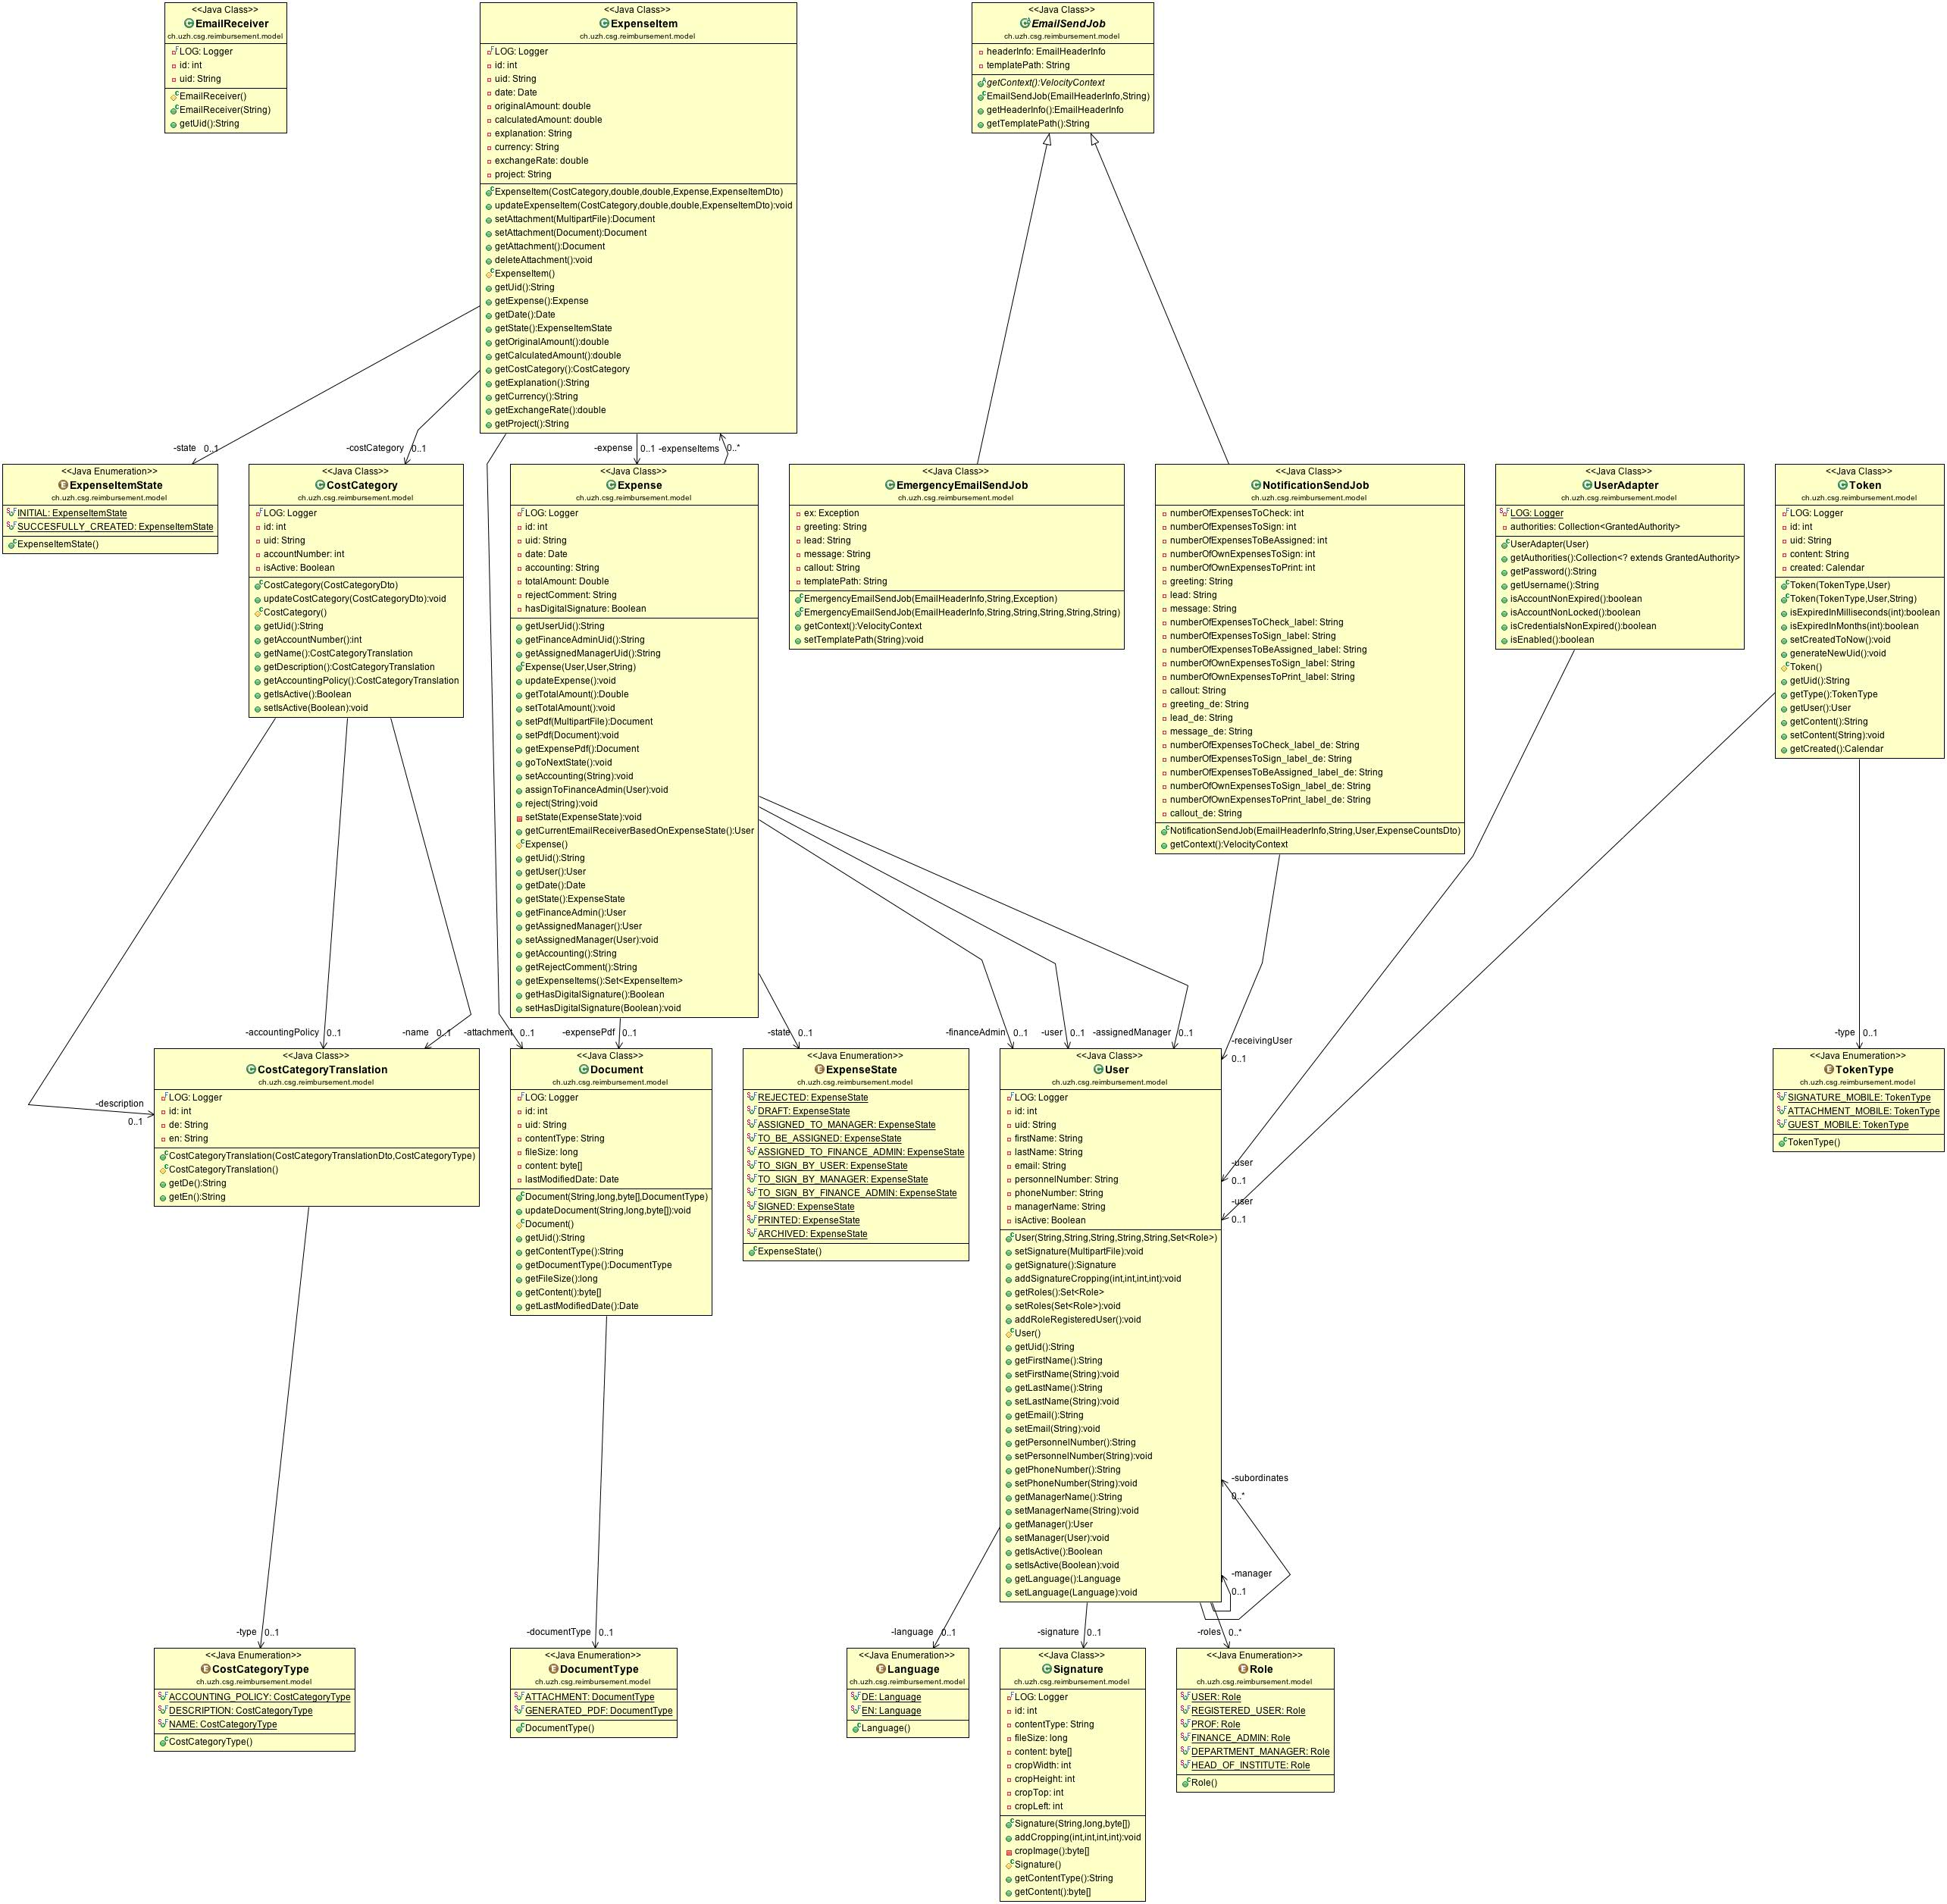
\includegraphics[width=1.0\textwidth]{umlclass-model}}
\end{figure}

\section{Services}
\label{sec:app-service}

\begin{figure}[H]
    {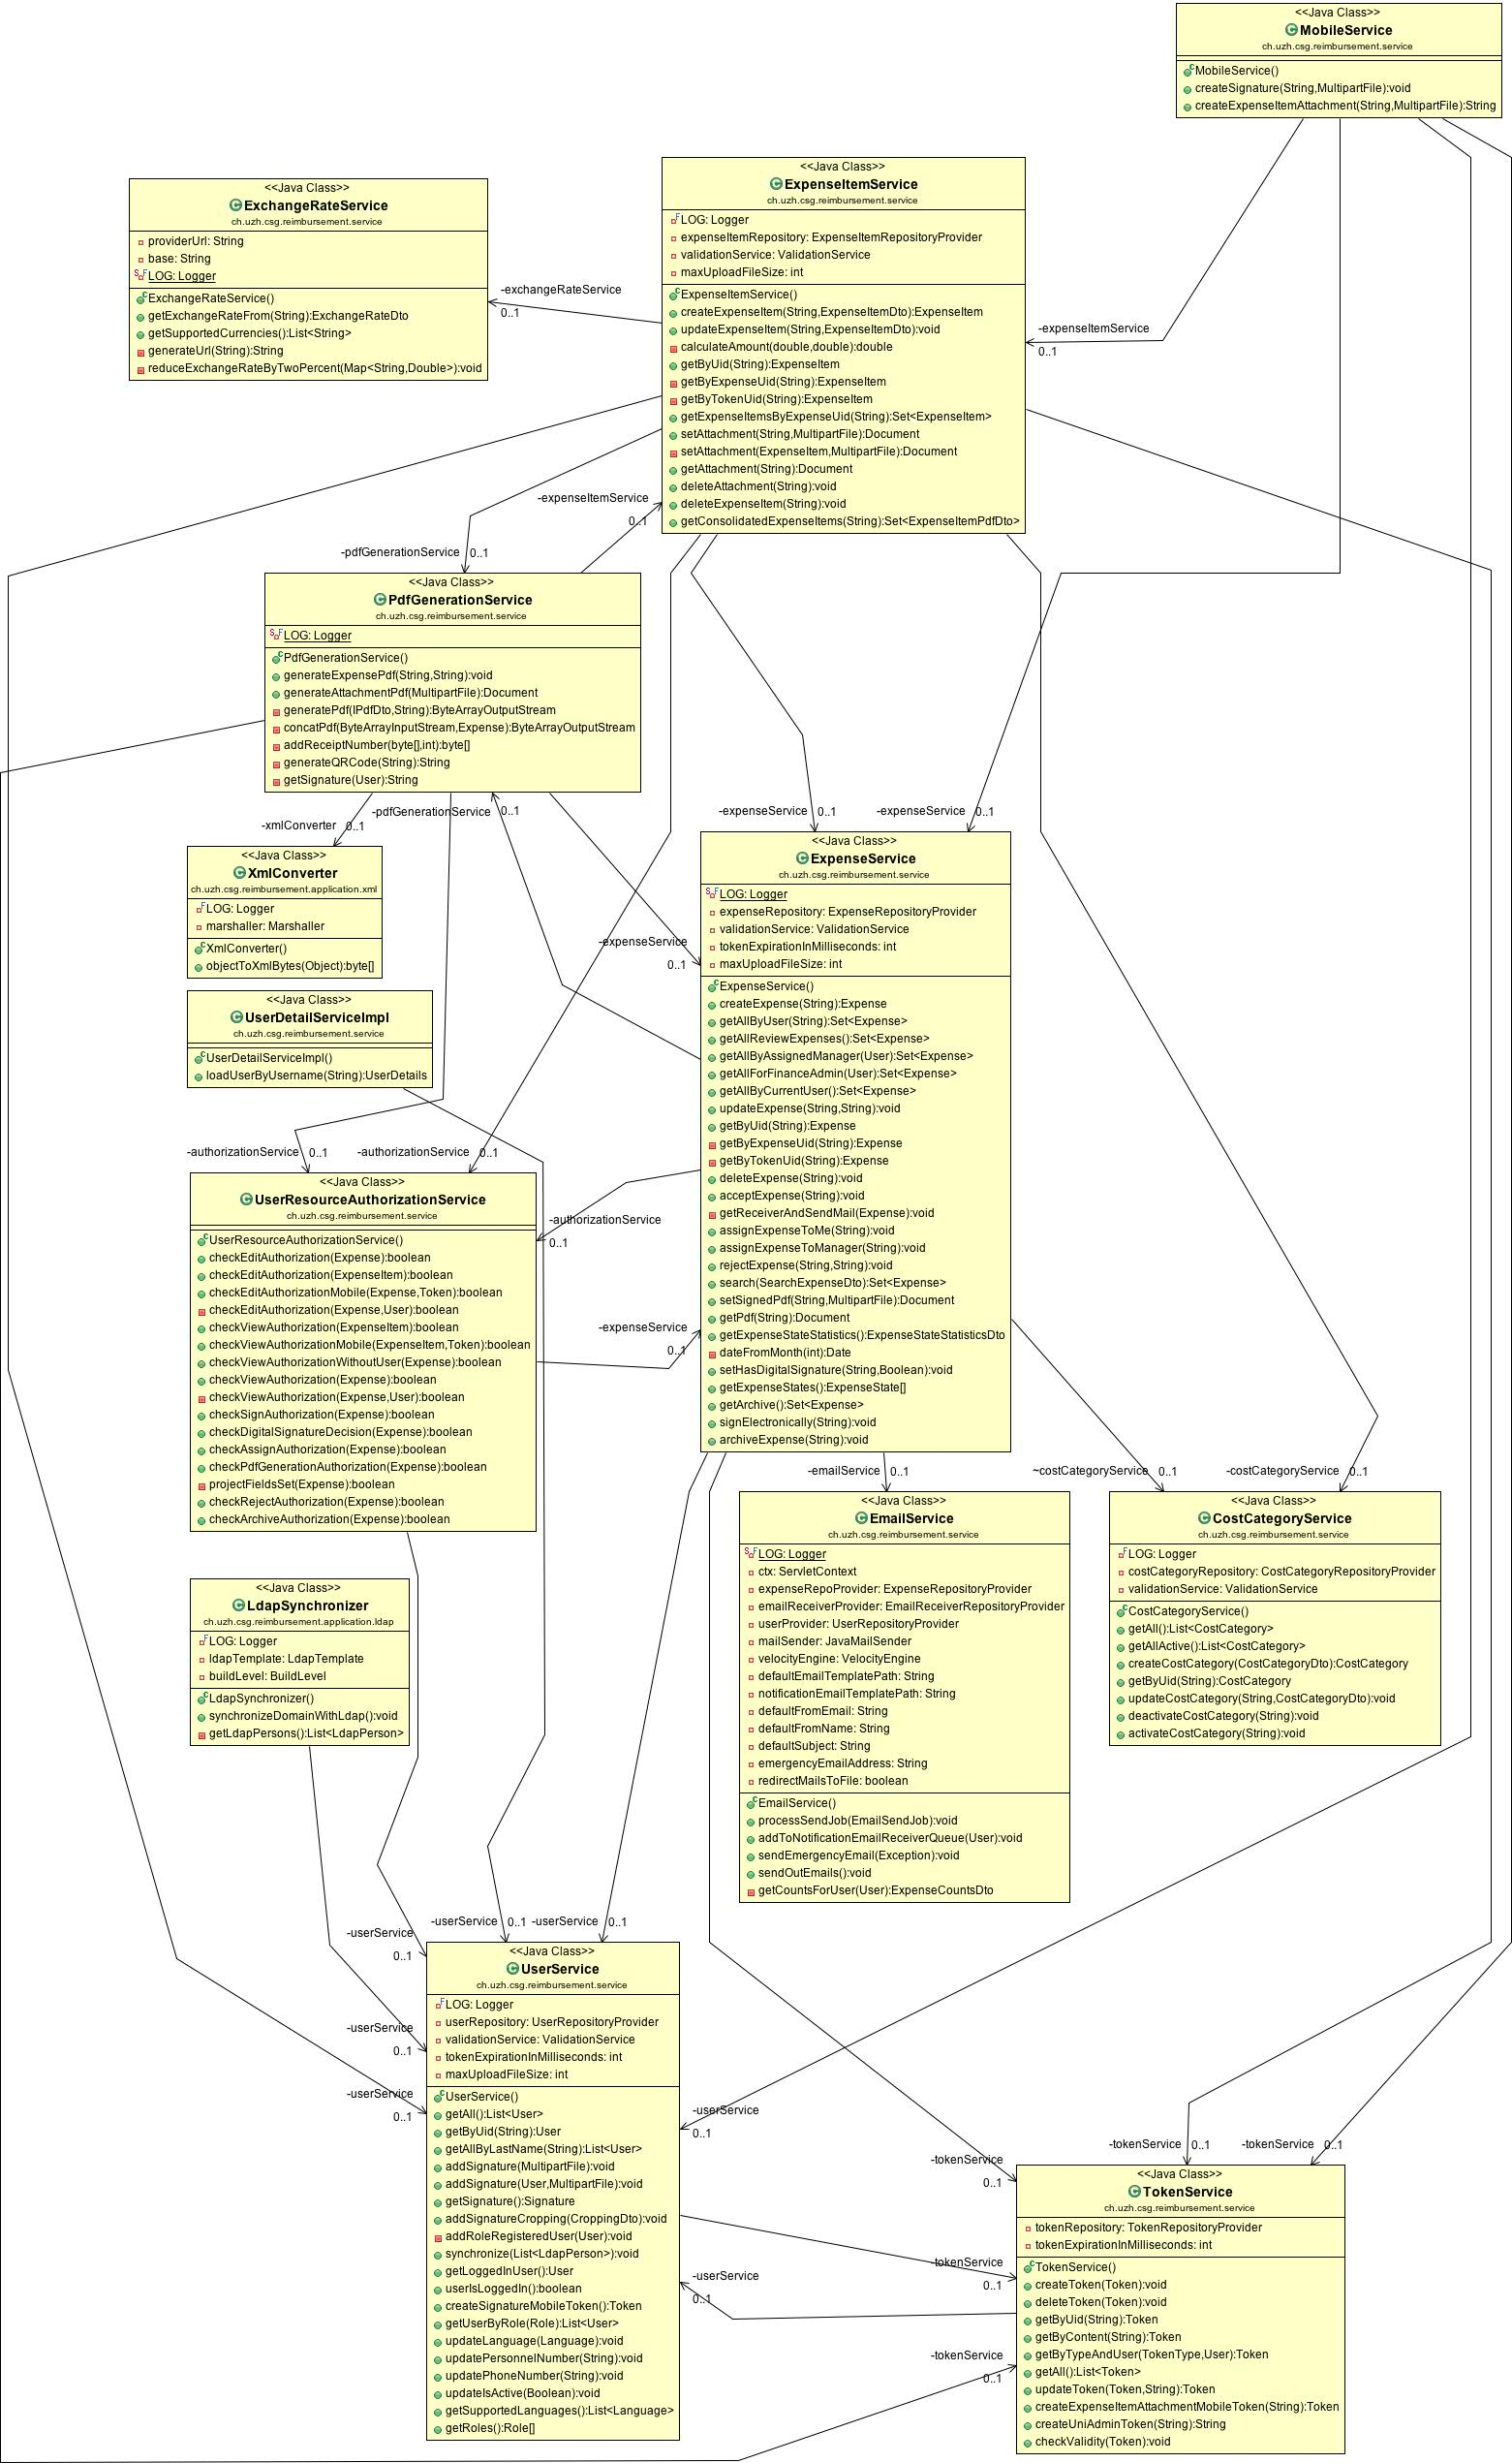
\includegraphics[width=0.95\textwidth]{umlclass-service}}
\end{figure}

\section{Process diagram}
\label{sec:process-diagram-rotated}

\begin{figure}[H]
    {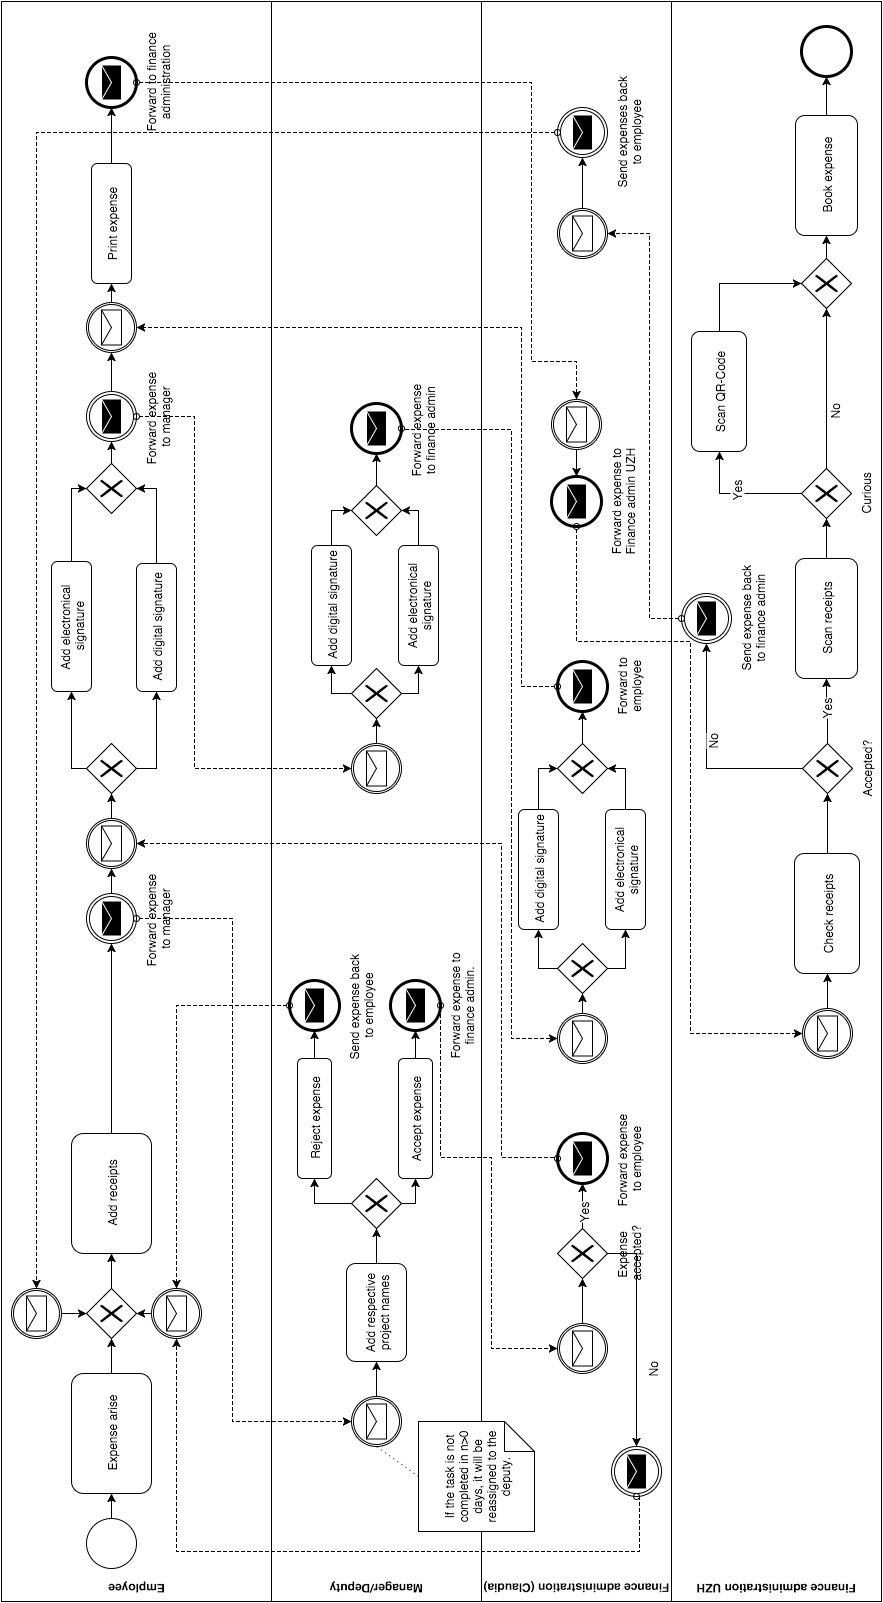
\includegraphics[width=0.8\textwidth]{process-diagram-rotated}}
\end{figure}

\section{State diagram}
\label{sec:state-diagram}

\begin{figure}[H]
    {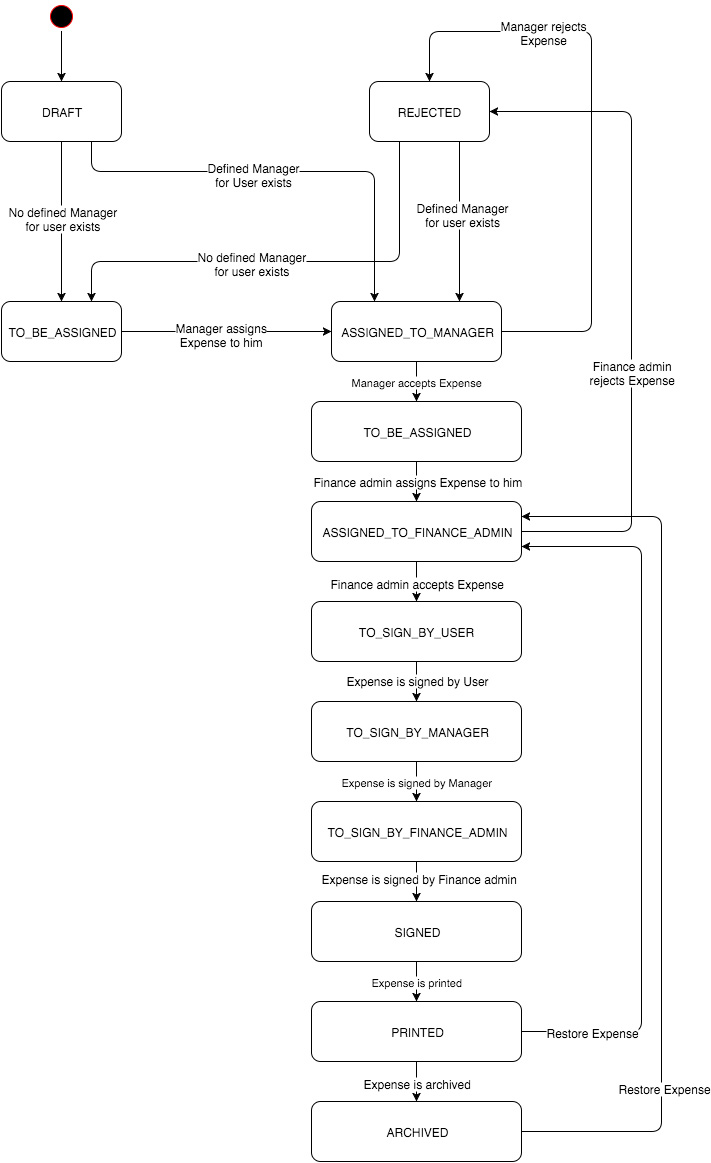
\includegraphics[width=0.8\textwidth]{state-diagram}}
\end{figure}

\section{PDF}
\label{sec:app-pdf}

\begin{figure}[H]
    {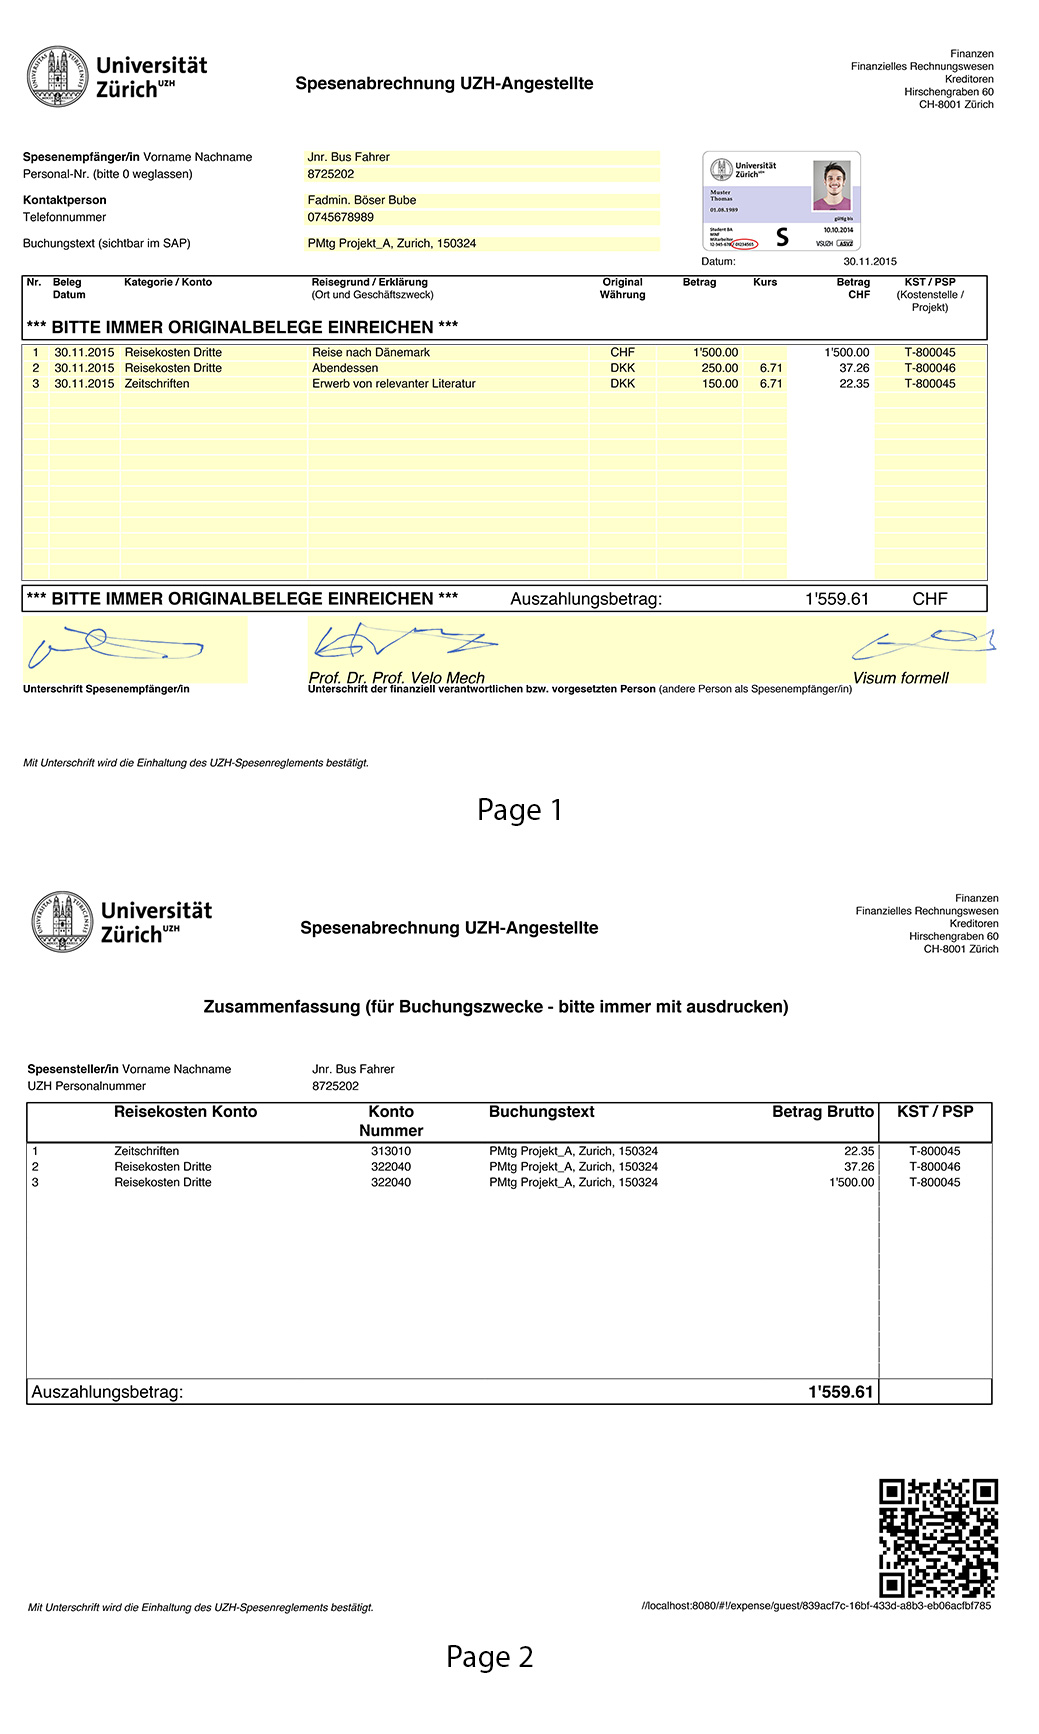
\includegraphics[width=0.95\textwidth]{pdf}}
\end{figure}

\chapter{Software source-code}
\label{github-source}

The complete software code is available on a public repository on \url{http://github.com}. There exists two repositories; one for the front-end and one for the back-end:

\begin{itemize}
\item Back-end: \newline \url{https://github.com/masterproject-reimbursement/reimbursement-server}
\item Front-end: \newline \url{https://github.com/masterproject-reimbursement/reimbursement-client}
\end{itemize}

For detailed installation instructions, please refer to appendix \ref{chap:installation}. 


\end{document}
